
\subsection{Experiments description}
In this section we compare the decomposition algorithm (both with Armijo and exact line search) against SNOPT \cite{snopt}.
The decomposition algorithm is written in \textit{Python 2.7} while we use the official Python interface for SNOPT. We also use \texttt{numpy} library, linked with \texttt{blas} and \texttt{ATLAS} libraries. The PC used for the experiments is equipped with and Intel i7 3630QM processor, 8GB of RAM and a Linux based distribution.\\
In order to obtain comparable results, in our scheme we use a \textit{stop criterion} that is the same used by SNOPT, i.e. we stop the algorithm when
\begin{equation}
\left| \frac{\partial f(x^k,y^k)}{d{x_{j(k)}}} - \frac{\partial f(x^k,y^k)}{d{x_{i(k)}} }\right| < \epsilon
\end{equation}
In SNOPT, this is (almost) equivalent to set the \texttt{Major optimality tolerance} optional parameter to $\epsilon$. 
In all the following experiments we used the NASDAQ-2196 dataset \cite{nasdaq}; from the covariance matrix contained in the dataset, we compute the correlation matrix and we use that instead of the covariance one for numerical reasons.
All the results are reported for $\epsilon = 10^{-10}$. This value of $\epsilon$ is such that the obtained solutions $(x^*,y^*)$ satisfies
\begin{equation}\label{eq:reseps}
\max_i \left| \frac{RC_i}{\mathcal{R}(x^*,y^*)} - \frac{1}{n} \right| < 10^{-6}
\end{equation}
where $RC_i$ is the risk contribution of the asset $i$ and ${\mathcal{R}(x^*,y^*)}$ is the total risk of the invested portfolio. Equation (\ref{eq:reseps}) express the fact that the (normalized) max deviation from Risk Parity of the solutions is less than $10^{-6}$.

\begin{figure}
\begin{minipage}{\linewidth}
\makebox[\textwidth][c]{
\begin{tikzpicture}
\begin{axis}[%
width=0.8\textwidth,
xlabel={\# of assets},
ylabel={Exe Time (s)},
legend pos=north west,
title=\textbf{Average execution time with {$\epsilon=10^{-10}$}},
]
\addplot [color=blue,solid,mark=x,mark options={solid}]
  table[row sep=crcr]{%
100	.148\\
200	.346	\\
300	.583	\\
500	1.486	\\
750	3.147		\\
1000 6.431 \\
1250 11.57 \\
1500 18.6\\
};
\label{Subplot:exe_e6_exact}

\addplot [color=red,solid,mark=x,mark options={solid}]
  table[row sep=crcr]{%
100	 .101   \\
200	 .269	\\
300	 .481	\\
500	 1.417	\\
750	 3.763	\\
1000 8.72  \\
1250 17.16 \\
1500 28.75 \\
};
\label{Subplot:exe_e6_armijo}

\addplot [color=gr,solid,mark=x,mark options={solid}]
  table[row sep=crcr]{%
100	.008		\\
200	.028		\\
300	.074	    \\
500	.353	    \\
750	 1.197  \\
1000 3.15	\\
1250 6.617	\\
1500 11.765 \\
};
\label{Subplot:exe_e8_snopt}
\addlegendentry{Exact LS}
\addlegendentry{Armijo LS}
\addlegendentry{SNOPT}
\end{axis}
\end{tikzpicture}
}
\end{minipage}

\begin{minipage}{\linewidth}
\makebox[\textwidth][c]{
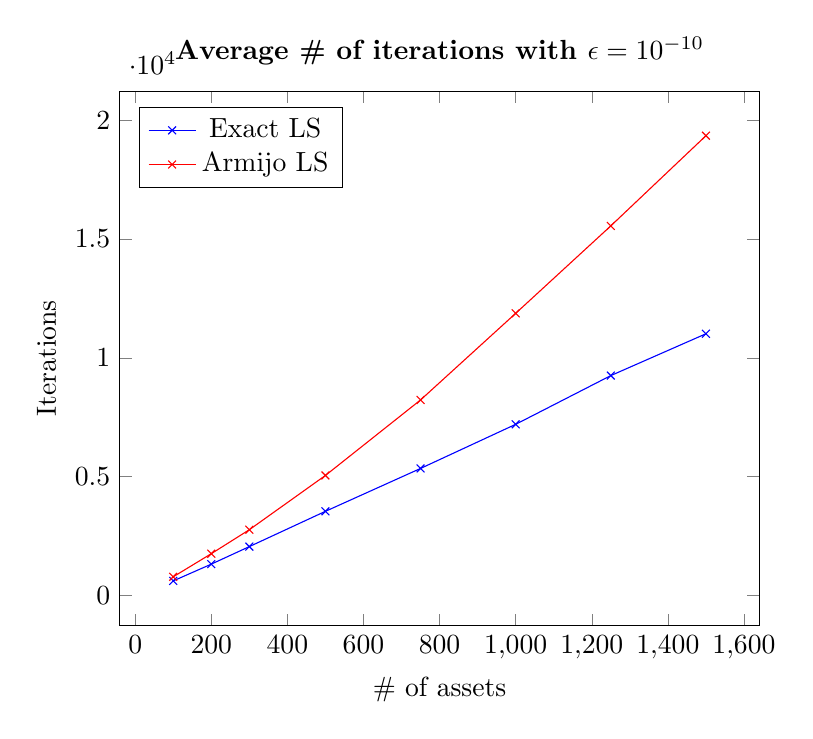
\begin{tikzpicture}
\begin{axis}[%
width=0.8\textwidth,
xlabel={\# of assets},
ylabel={Iterations},
legend pos=north west,
title=\textbf{Average \# of iterations with {$\epsilon=10^{-10}$}}
]
\addplot [color=blue,solid,mark=x,mark options={solid}]
  table[row sep=crcr]{%
%50	242\\
%75	379\\
100	609 \\
200	1315 \\
300	2053 \\
500	3538\\
750	5343 \\
1000	7200\\
1250	9251\\
1500    11011\\
};

\addplot [color=red,solid,mark=x,mark options={solid}]
 table[row sep=crcr]{%
%%50	309    \\
%%75	483    \\
100	782    \\
200	1754		\\
300	2763		\\
500	5048		\\
750	8225		\\
1000	 11871	\\
1250	 15552	\\
1500	 19347\\
};

\addlegendentry{Exact LS}
\addlegendentry{Armijo LS}
\end{axis}
\end{tikzpicture}
}
\end{minipage}
\label{perf}
\end{figure}

\begin{table}
\begin{minipage}{.4\linewidth}
\centering
\begin{tabular}{ c | c | c | c }
n &  G-S$_{(LS)}$ & G-S$_{(OPT)}$  & SNOPT \\\hline
5    & 100.0\% & 100.0\% & 100.0\%\\\hline
10   & 100.0\% & 100.0\% & 100.0\%\\\hline
20   & 100.0\% & 100.0\% & 100.0\%\\\hline
50   & 99.0\%  & 99.4\%  & 99.5\%\\\hline
100  & 85.4\%  & 87.0\%  & 91.2\%\\\hline
200  & 40.0\%  & 45.0\%  & 52.0\%\\\hline
300  & 22.0\%  & 24.0\%  & 34.0\%\\\hline
500  & 0.0\%   & 6.0\%   & 3.0\%\\\hline
750  & 0.0\%   & 2.0\%   & 0.0\%\\\hline
1000 & 0.0\%   & 0.0\%   & 0.0\%\\\hline
1250 & 0.0\%   & 0.0\%   & 0.0\%\\\hline
\end{tabular}
\caption{$x^{0}_i = 1/n \quad \forall i$}
\end{minipage}
\hfill
\begin{minipage}{.4\linewidth}
\centering
\begin{tabular}{ c | c| c | c}
n &  G-S$_{(LS)}$ & G-S$_{(OPT)}$  & SNOPT \\\hline
5    & 100.0\%  & 100.0\% & 100.0\%\\\hline
10   & 100.0\%  & 100.0\% & 99.9\%\\\hline
20   & 100.0\%  & 100.0\%  & 100.0\%\\\hline
50   & 100.0\%  & 99.9\%  & 99.9\%\\\hline
100  & 99.9\%   & 100.0\%  & 99.6\% \\\hline
200  & 100.0\%  & 100.0\%  & 98.8\% \\\hline
300  & 100.0\%  & 100.0\%  & 96.6\% \\\hline
500  & 99.5\%   & 99.2\%   & 88.0\%\\\hline
750  & 99.5\%   & 99.2\%  & 83.0\%\\\hline
1000 & 98.0\%   & 95.2\%  & 83.0\%\\\hline
1250 & 91.5\%   & 93.2\%  & 73.0\%\\\hline
\end{tabular}
\caption{$x^{0}= [1, 0, .., 0]$}
\end{minipage}
\end{table}
